\section{Optical properties of the sphere }
\label{sec:opt}

The central component of the experiment is the HPFS sphere, which holds the LXe target, located in the center 
of the detector system. The sphere is made of two Corning HPFS 8655 hemispheres attached by a UV transparent glue. 
The refractive index of this HPFS is 1.58 at 185 nm, matching to the LXe one, which is 1.61. Hence, there is minimal 
diffraction from the original direction of the photons as they transit from the LXe target to the sphere. The refractive 
indexes at various wavelengths are shown in Fig.~\ref{fig:hpfsRIcalibration} (left panel).


<<<<<<< HEAD
The HPFS transparency to VUV photons is an extremely crucial parameter for setting the sphere's dimensions (inner and outer radii). 
Therefore, the transmittance of an HPFS sample was measured, using a VUV monochromator light source. 
The measured transmittances as a function of wavelength are shown in Fig.~\ref{fig:hpfsRIcalibration}~(right panel). The 
transmittance of the sample at 178~\,nm, is$\sim98.7$\,\%/cm.  
=======
The HPFS transparency to VUV photons is an extremely crucial parameter for setting the sphere's dimensions (inner and outer radii) and detector sensitivity. Therefore, the transmittance of an HPFS sample was measured, using a VUV monochromator light source. 
The measured transmittances as a function of wavelength are shown in Fig.~\ref{fig:hpfsRIcalibration}~(right panel). The \sout{intrinsic} transmittance of the sample at 178~\,nm, is$\sim98.7$\,\%/cm.  
>>>>>>> 2292d93adb63079752489fa3b355837dcdd54054

\begin{figure}[h]
   \centering
   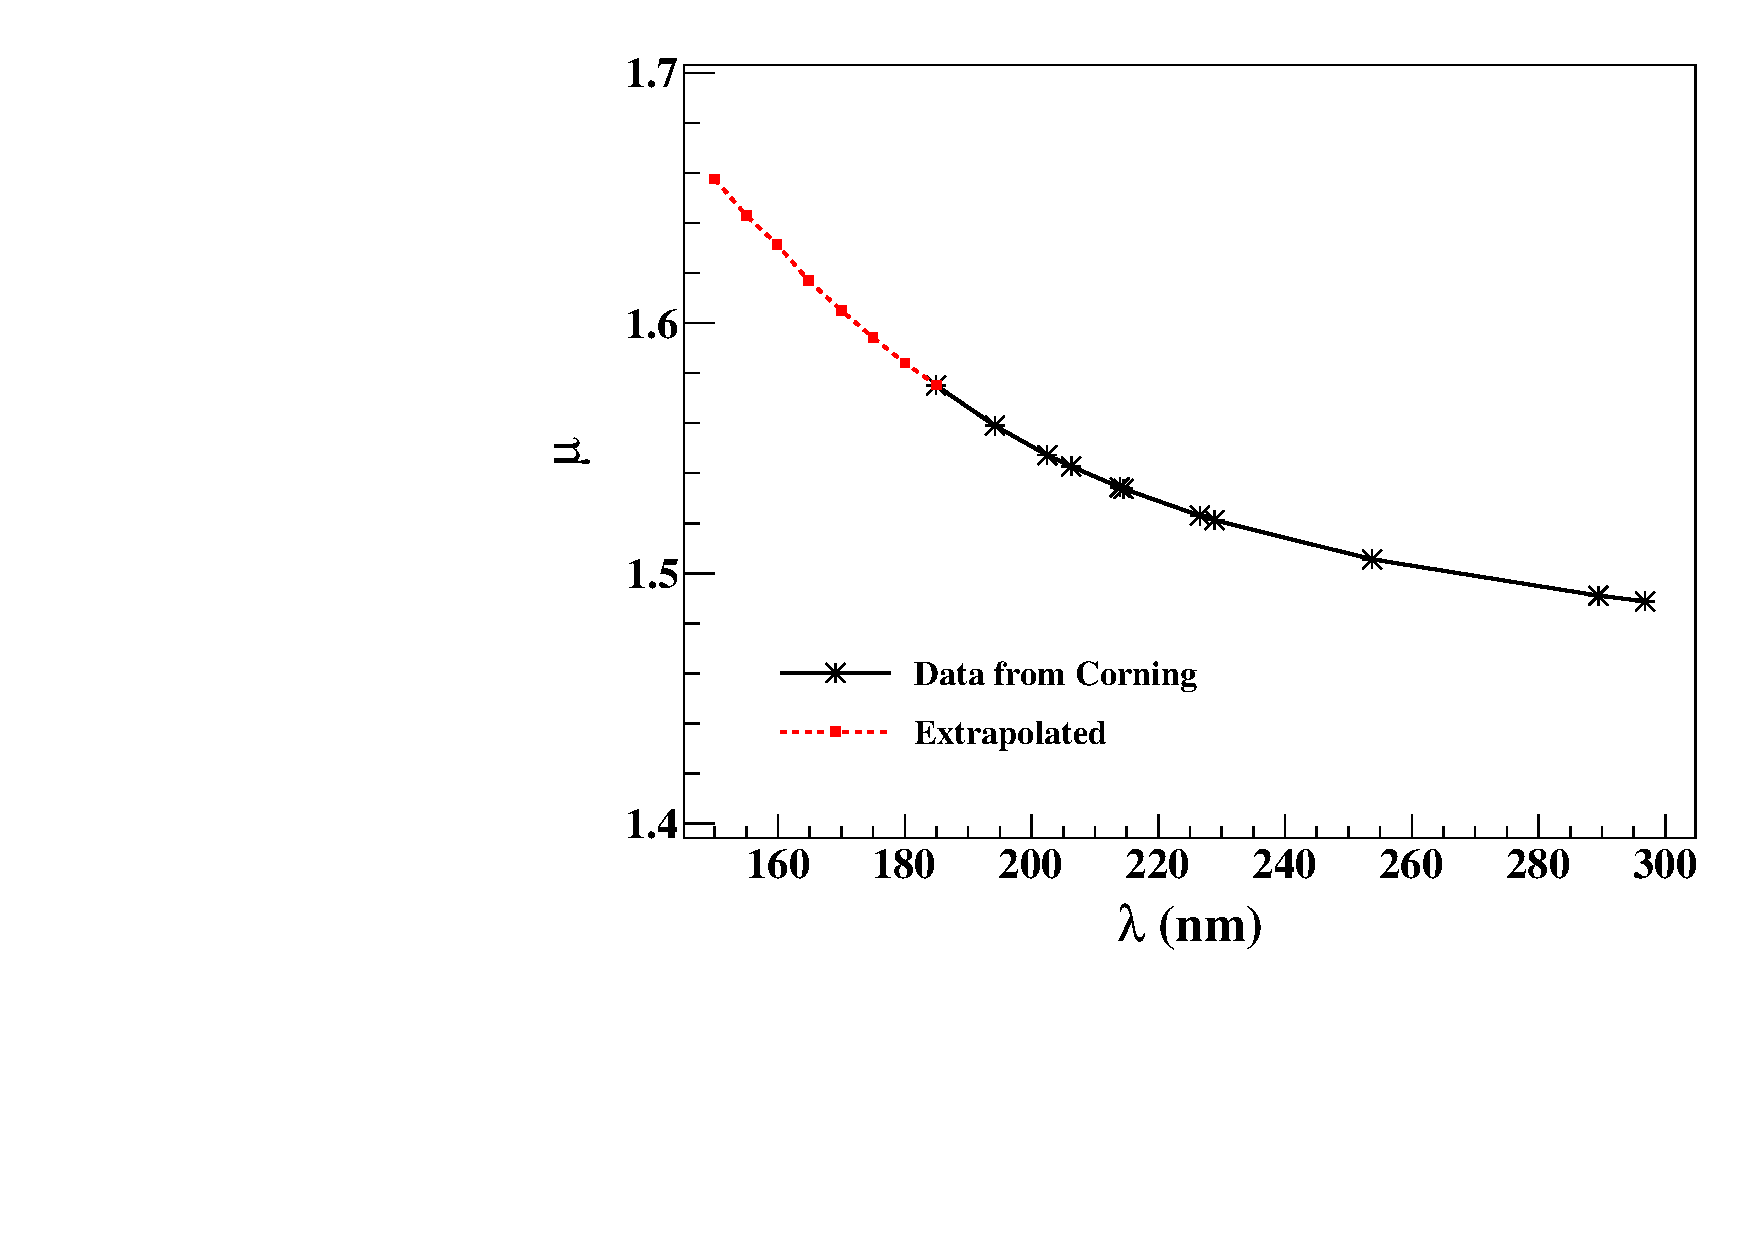
\includegraphics[width=0.48\textwidth]{RI-calibration.pdf}
    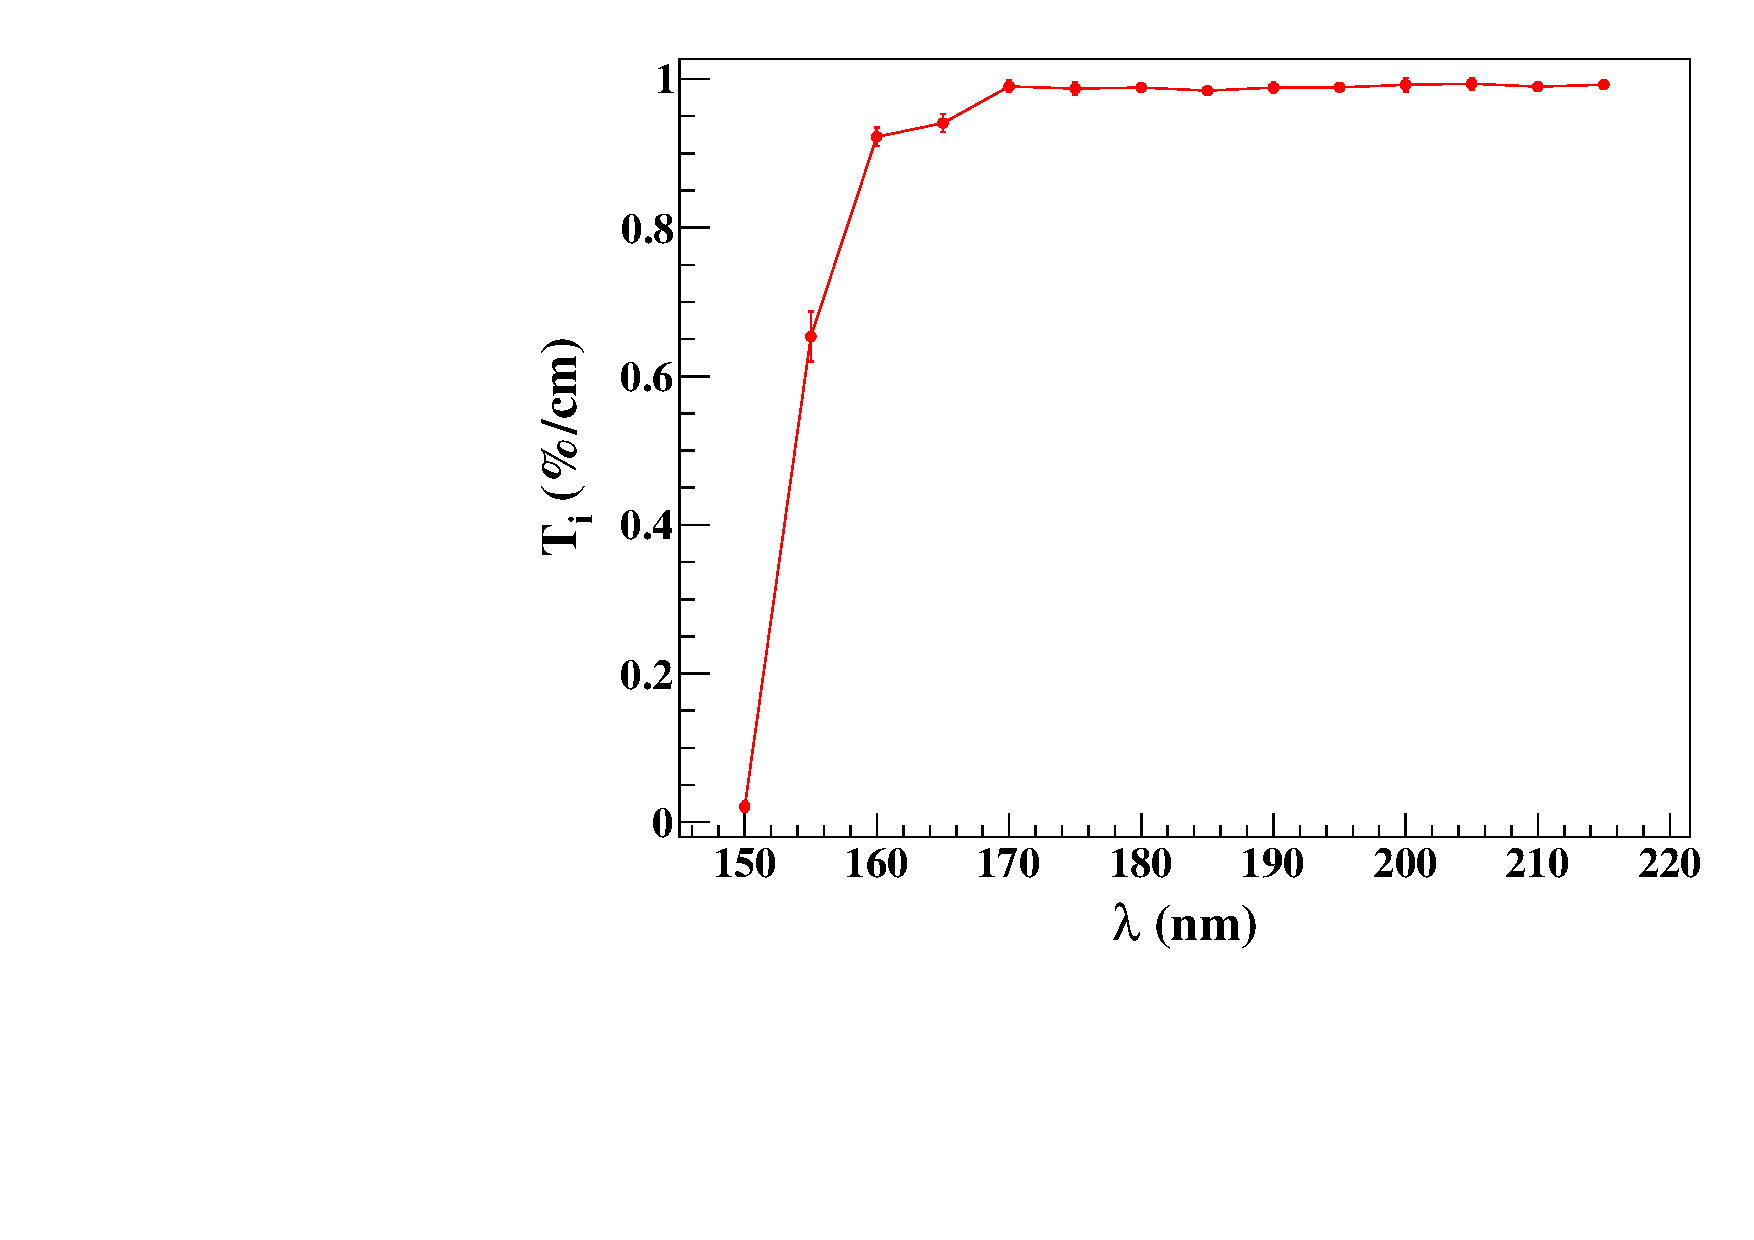
\includegraphics[width=0.48\textwidth]{IntTransmittance.pdf}
   \caption{Some relevant characteristics of HPFS-8655. (Left) The refractive index as provided by corning and 
   extrapolated to relevant wavelength range. (Right) The internal transmittance ($T_{i}$).} 
   \label{fig:hpfsRIcalibration}
\end{figure}


The shell should be thick enough to reduce internal reflections, but not 
<<<<<<< HEAD
too thick to attenuate the scintillation light and the LXe target bubble within it should not be too large in order to avoid double scatters. 
The sources that will be used for exciting the xenon, and creating the supperradiance 
=======
too thick to attenuate the scintillation light. The LXe target bubble within should not be too large in order to avoid double scatters. The sources that will be used for exciting the xenon, and creating the supperradiance 
>>>>>>> 2292d93adb63079752489fa3b355837dcdd54054
(signal) as well as the standard emission (background), will be $^{137} \mathrm{Cs}$ 
(E$_\gamma$=662 keV) and $^{57} \mathrm{Co}$( E$_\gamma$= 122keV \& 136 keV) for ER with mean free path of $\sim4$\,cm and $\sim1$\,cm respectively. For NR $^{241}$AmBe , 
D-D neutron generator, or neutron produced in an accelerator will be used.

Using a GEANT4 based simulation~\cite{AGOSTINELLI2003250} studying the path of the scintillation photons the sphere dimensions are optimized. 
The outer radius  is 3 cm, and the inner (the hollow space that holds the LXe) is 1 cm. 
